\documentclass[10pt,twocolumn,letterpaper]{article}

\usepackage{cvm}
\usepackage{times}
\usepackage{epsfig}
\usepackage{graphicx}
\usepackage{amsmath}
\usepackage{amssymb}

\usepackage{stfloats}
\usepackage{setspace}

%数学命令
%\input{math-commands.tex}

% Include other packages here, before hyperref.

% If you comment hyperref and then uncomment it, you should delete
% egpaper.aux before re-running latex.  (Or just hit 'q' on the first latex
% run, let it finish, and you should be clear).
\usepackage[pagebackref=true,breaklinks=true,letterpaper=true,colorlinks,bookmarks=false]{hyperref}


% \cvmfinalcopy % *** Uncomment this line for the final submission

\def\cvmPaperID{****} % *** Enter the cvm Paper ID here
\def\httilde{\mbox{\tt\raisebox{-.5ex}{\symbol{126}}}}

% Pages are numbered in submission mode, and unnumbered in camera-ready
\ifcvmfinal\pagestyle{empty}\fi

\graphicspath{{figures/}}  % 图片存放路径

\begin{document}

%%%%%%%%% TITLE
\title{Effect of instance normalization on fine grained control in sketch-based face generalization}

\author{First Author\\
Institution1\\
Institution1 address\\
{\tt\small firstauthor@i1.org}
% For a paper whose authors are all at the same institution,
% omit the following lines up until the closing ``}''.
% Additional authors and addresses can be added with ``\and'',
% just like the second author.
% To save space, use either the email address or home page, not both
\and
Second Author\\
Institution2\\
First line of institution2 address\\
{\small\url{http://www.author.org/~second}}
}

\maketitle
% \thispagestyle{empty}

%%%%%%%%% ABSTRACT
\begin{abstract}
    In this paper we investigate the effect of instance normalization on fine grained control in generating photorealistic face images from hand-drawn sketches with data reduction and visualization methods. Exiting image-to-image translation methods mostly utilize instance normalization after activation as nomalization layer.
    But this induces the problem of missing some precise textures in the generated images and weakening face editing performance as we modify the input sketches. To address this issue, we improve upon baseline model on the network architecture. We show how a small change in the generator architecture results in a significant improvement of the image generation quality.  
    User studies demonstrate that our method surpass the baseline method regarding both face editing and image fidelity.
    
\end{abstract}

%%%%%%%%% BODY TEXT
\section{Introduction}
Photorealistic face image synthesis from hand-drawn sketches has drawn a lot of attention in computer graphics and computer vision for many years. The typical approaches use generative and adversarial networks(GANs)\cite{gan}, whose generator is built by stacking convolutional, normalization, and nonlinearity layers, as their network architectures. Normalization layers, in fact, can normalize the parameter distribution so as to alleviate the issue of slow convergence in gradient update process and avoid gradient disappearance and explosion, which is vastly important in GANs.

There are many normalization means with different goals, such as batch normalization\cite{bn}, group normalization\cite{gn}, layer normalization\cite{ln} and instance normalization\cite{instance_norm}. Batch normalization eliminates the influence of internal covariant shift, effectively avoids the possible problems of gradient disappearance and gradient explosion in the process of network parameter gradient backpropagation, and makes the convergence of the training process faster. Group normalization is frequently used in some tasks such as object detection, semantic segmentation and in some video-associated tasks. Layer normalization is more suitable for RNN and can be used in test phase.

Instance normalization\cite{instance_norm} has a remarkable effect on tasks such as style transfer and image translation\cite{pix2pixhd,spade,cyclegan}. In fact, instance normalization is very similar to batch normalization, with the only difference being that batch normalization computes the mean and variance of all feature maps within a batch, while instance normalization only aim at a single sample. Instance normalization only considers the information of a single channel in a sole image, which is more suitable for per pixel tasks such as image translation. Nonetheless, instance normalization layers also tend to "wash sway" information contained in the input sketches, thus lead to descent of the feature expression ability and imprecise control on detailed texture generation. 

We investigate the effect of instance normalization on fine grained control in sketch-based photorealistic face image generation using data reduction and visualization methods. We utilize PCA and t-SNE to visualize and analyze features extracted by the generator from sketches. Consequently, we propose to remove the first two instanse normalization layers in the baseline generator, and we show how a small change in the generator architecture results in a significant improvement of control accuracy in the image generation. We conduct experiments and interactive user study to evaluate our proposed method, and the results demonstrate that our method surpass baseline method on control performance on the sketch-to-image task.

\section{Related Work}
\subsection{Image-to-Image Translation}
The goal of image-to-image translation\cite{pix2pix} task is to convert the input images from one domain to another given the input-output image pairs as training data, in other words, to generate corresponding images in the other domain according to the input images, and meanwhile the two images share the same structure and scene. At present, many researchers employ adversarial manner to train deep neural networks in image translation tasks\cite{sis,cfgan,spade}.

The concept of image-to-image translation was first proposed by pix2pix\cite{pix2pix}, which is based on generative adversarial networks conditioned on images. The network architecture of \cite{pix2pix} is composed of generator $G$ and discriminator $D$, the former is responsible for converting the input image from source domain to target domain, and the latter is responsible for telling the generated image apart from the real image. This model can be applied to a variety of different image translation scenarios, such as lable maps to streetscapes, edge maps to photos and image colorization.
However, the defect of pix2pix is also obvious. At most, it can only generate images with a resolution of 256 × 256. If forced to use pix2pix to generate images with a higher resolution, the training process will be unstable and the generation quality will decline. Therefore, T. Wang et al. proposed a new image-to-image translation model referred to as pix2pixHD\cite{pix2pixhd}, which is based on pix2pix, aiming to improve the resolution of generated image from semantic lable maps. It adopts a coarse-to-fine generator and a multiscale discriminator. It can also be applied to edge-to-photo generation condition on edge map and photo pairs. However, the large gap between synthesized edge maps and hand-drawn sketches challenges the generalization of these models.

\subsection{Normalization Layers}
Normalization layers have been an important component in modern deep neural networks in order to stabilize the training process. The following are several common normalization methods.Batch normalization\cite{bn} eliminates the influence of internal covariant shift, effectively avoids the possible problems of gradient disappearance and gradient explosion in the process of network parameter gradient backpropagation, and makes the convergence of the training process faster. Group normalization\cite{gn}, evidently, group the channels of feature maps and normalize each group of elements with mean 0 and standard deviation 1, which is frequently adopted in some tasks such as object detection, semantic segmentation and in some video-associated tasks. Layer normalization\cite{ln} is more suitable for RNN and can be used in test stage. Instance normalization\cite{instance_norm} has a remarkable effect on tasks such as style transfer and image translation. It is used in the baseline method\cite{pix2pixhd} and other image translation tasks\cite{spade,cyclegan}. In fact, instance normalization is very similar to batch normalization. The only difference is that batch normalization computes the mean and variance of all feature maps within a batch, while instance normalization only considers a single sample. So instance normalization is more suitable for per pixel tasks such as image translation.

\section{Methods}

\subsection{The pix2pixHD Baseline}
Pix2pixHD\cite{pix2pixhd} is an image translation model based on conditional generative adversarial network, which can generate high-quality and high-resolution images from input semantic label maps. It adopts a improved adversarial loss, as to the network architecture it introduces a coarse-to-fine generator and a multiscale discriminator. Using this model, a more realistic image with a resolution of 2048 × 1024 can be generated, which is better than the previous method. In addition, the model can also be used for interactive image editing. First of all, we can add the instance segmentation information of the object into the input to realize the editing of the object, such as adding or deleting objects or changing the category of objects in the generated image. Second, you can edit the appearance of an object in the generated image given the same input. 

Its generator is divided into two sub networks: $G_1$ and $G_2$. $G_1$ is alled global generator network, and $G_2$ is called local enhancer network, where $G_1$ is used to generate base image, and $G_2$ is used to improve the resolution of the image. In order to distinguish real and generated images with high resolution, the discriminator needs to have a large perception field. Therefore, the model uses a multi-scale discriminator which can preserve both global and local information. The loss function of this model is composed of three parts: adversarial loss $L_{GAN}(G,D_k)$, feature matching loss $L_{FM}(G,D_k)$ and VGG perceptual loss $L_{VGG}(G)$. The full objective is formulated as:
\begin{equation}
\begin{split}
	&\underset{G}{\min}\Bigg(\bigg(\underset{D_1,D_2,D_3}{\max} \sum_{k=1,2,3}{L_{GAN}\big(G,D_k\big)}\bigg)+  \\
	&\lambda \bigg(\frac{1}{3}\sum_{k=1,2,3}{L_{FM}(G,D_k)}+L_{VGG}{\big(G(\boldsymbol{s})\big)}\bigg)\Bigg)~.
\end{split}
\end{equation}
\noindent
where $\lambda$ controls the importance of the three terms.

\subsection{Network Architecture}
In generator, the activation of convolutional output is normalized in the channel-wise manner and then modulated with unified scale and bias within channel. This operation, to a certain extent, leads to a negative effect that a local change in the input sketch broadcasts globally, thus resulting in a degraded capacity of fine-grained control on generated image.
 
However, the gradient disappearance or explosion is bound to emerge when the instance normalization layers in feature extraction stage of the generator network is abandoned too much, which makes the training process difficult to converge. Based on the consideration above, we remove the first two instance normalization layers in the global generator of pix2pixHD baseline and take the rest as our own generator. The architecture of our generator is shown in Fig.~\ref{fig:our_generator}~. Our generator operates at a resolution of 512×512. It consists of 4 components: a convolutional front-end without normalization $G_1^{(F)}$, a down-sampled convolutional mid-end $G_1^{(M)}$, a set of residual blocks $G_1^{(R)}$ and a transposed convolutional back-end $G_1^{(B)}$. $G_1^{(F)}$ composed of two unnormalized convolution and activation layers can remain underlying information of input sketches locally, scilicet information flowing through the network without broadcasting. Hence efficient fine-grained control on generated images can be conduct. %we use the global generator of pix2pixHD baseline without the first two instance normalization layers as our own generator.%
\begin{figure*}[htbp]
	\centering
	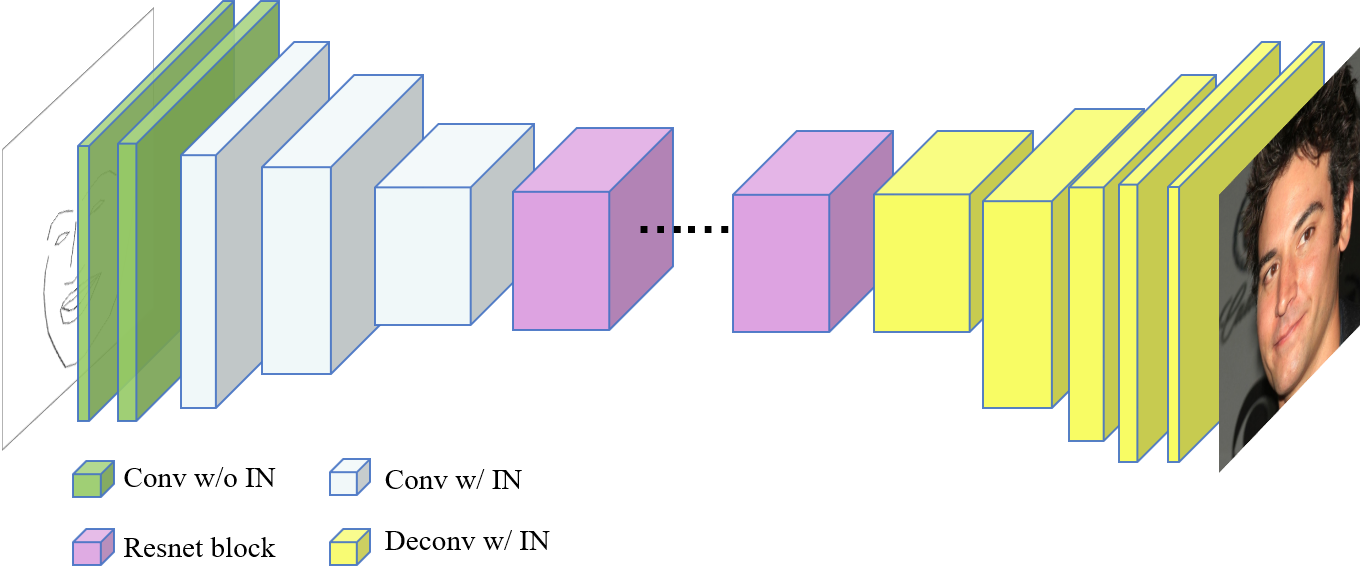
\includegraphics[width=0.8 \textwidth]{our_model_G.png}
	\caption{Network architecture of our generator. }
	\label{fig:our_generator}
\end{figure*}

The discriminator applys the multi-scale design consistent with pix2pixHD. There are 3 discriminators that have an identical network structure but operate at different image scales. In addition, each discriminator is built on PatchGAN architecture proposed by Isola Phillip \textit{et al.}\cite{pix2pix}. Sketches at different scales are concatenated with corresponding face images, and fed into the discriminators, respectively. 

\section{Experiment}
We conduct extensive experiments to evaluate our proposed method.
In Sec.~\ref{sec:visualize}, we visualize the feature vectors extrcted from hand-drawn sketches by the generator of pix2pixHD baseline and our model, and analyze the visualization results to investigate the effect of instance normalization on fine grained control in generated face images.
In Sec.~\ref{sec:results}, we introduce how to produce our training and testing datasets. Next we introduces the method of data augmentation aiming to alleviate the problem that the generated image has poor tolerance to the spatial position change of the input sketches, and shows the generation results of the model trained with augmented data. Further more, we conduct comparative experiments on hand-drawn sketches between our methods and pix2pixHD baseline.

\subsection{Feature Visualization}\label{sec:visualize}
We extract the feature vector of the middle layers of the generator network and analyze them using two data visualization tools comparatively.

\noindent
$\mathbf{Feature ~vector ~extraction}$ In order to verify whether the existing image translation neural network can extract the face shape features consistent with the user's intention for the hand-drawn sketches with low accuracy and geometric deformation, we draw 198 sketches of resolution $512\times512$. Fig.~\ref{fig:hand_drawn_contours}~ shows examples of these 11 sets of hand-drawn sketches.  
\begin{figure*}[htbp]
	\centering
	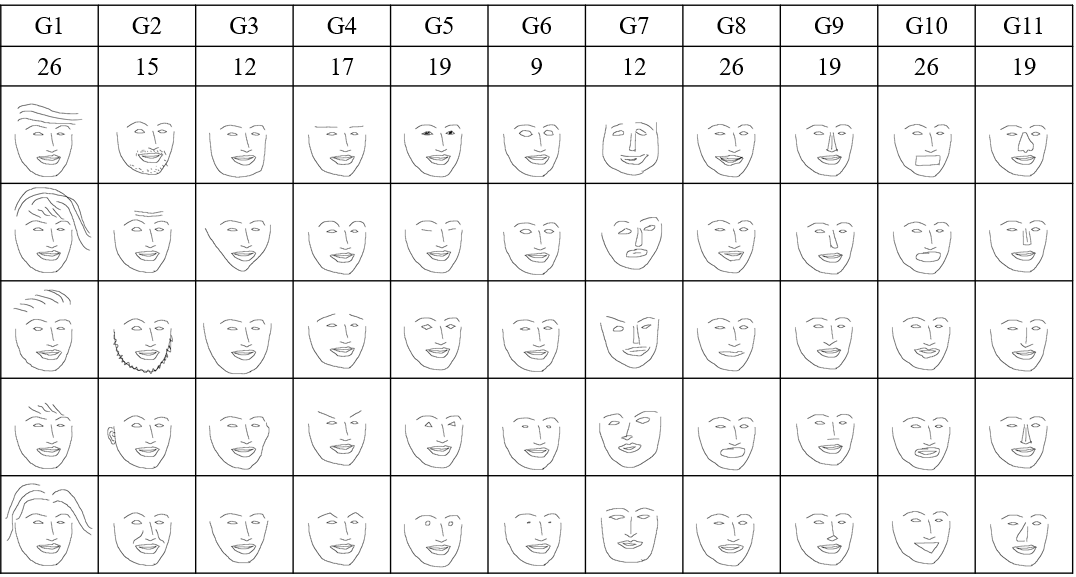
\includegraphics[width=0.9 \textwidth]{hand_drawn_sketches.png}
	\caption{These sketches can be divided into 11 categories. G1:Add hair; G2:Add new attributes, such as whiskers, wrinkles, ears; G3:Change face shape; G4:Change eyebrows; G5:Change eye shape; G6:changes eye size; G7:Graffiti-drawn; G8:Change mouth; G9:Change nose; G10:Change mouth(same eyes as G9); G11:Change nose(same eyes as G8). Specifically, there is no correlation between G7 and the other 10 classes. Except G7, the sketch only changes a particular location or property while the rest of the sketch remains the same. Except for the same eye between G8 and G11, G9 and G10, the eye lines of other categories of sketches are different.}
	\label{fig:hand_drawn_contours}
\end{figure*}

We refer to the first 5 layers of our generator as $L_0,\ldots,L_4$. With the hand-drawn sketches fed into the generator, we get 5 feature maps as output of $L_0$ to $L_4$, and then we extract one full channel feature vector on the left eye corner point of coordinate (170, 250) from each of the 5 feature maps respectively. We call the 5 vectors $\boldsymbol{v}_k,~k=0,\ldots,4$. The coordinates of the corresponding points on the five feature maps are (170, 250), (85, 125), (43, 63), (22, 32) and (11, 16). And the perceptive fields of the 5 vectors are $7\times7$, $9\times9$,$13\times13$, $21\times21$ and $37\times37$ as shown in Fig.~\ref{fig:receptive}. The dimensions of these 5 feature vectors are 48, 96, 192, 384 and 768, respectively. We get the 5 feature vectors of pix2pixHD generator called $\boldsymbol{v}_0^{'},\ldots,\boldsymbol{v}_4^{'}$ in the same way.
\begin{figure}[htbp]
	\begin{center}
	%\centering
	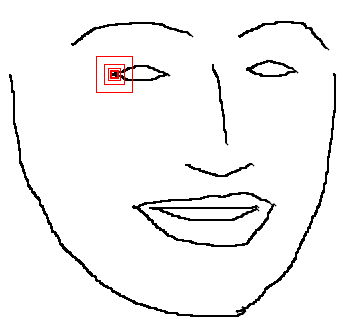
\includegraphics[width=0.2 \textwidth]{receptive_field.png}
	\end{center}
	\caption{The perceptive fields of corresponding left eye corner points in the feature maps $L_0\sim L_4$. }
	\label{fig:receptive}
\end{figure}

\noindent
$\mathbf{Visualization ~with ~PCA}$ Principal Component Analysis (PCA)\cite{pca} is a common linear data dimension reduction method, which can better retain the statistic characteristics of data in high dimensional space. We use PCA to perform visually analysis on $\boldsymbol{v}_0\sim \boldsymbol{v}_4$ after dimension reduction.
Fig.~\ref{fig:pca_1}(a) and Fig.~\ref{fig:pca_1}(b) demonstrate the results of PCA visualization on $\boldsymbol{v}_0$ and $\boldsymbol{v}_1$, and Fig.~\ref{fig:pca_1}(c) is a legend which is applicable to the following chapters. The corresponding relationship between hand-drawn sketch categories and number colors are: G1 (light blue), G2 (light purple), G3 (pale red), G4 (blue), G5 (orange), G6 (olive green), G7 (pink), G8 (gray), G9 (purple), G10 (light green), G11 (yellow).
It can be seen from the figure that the data of G1, G2, G3 and G4 are distributed at a same point respectively, the data of G8 and G11 are gathered on the same point, the data of G9 and G10 are distributed at the same point, whereas the data of G5, G6 and G7 are distributed dispersedly. 
This indicates that after the removal of the instance normalization in the first two layers, the features of the left eye corner point are only affected by the contents of the sketch in the corresponding perceptive field, and the change of the sketch in the perceptive field will change the extracted features of the corresponding points but will not beyond the perceptive field.
\begin{figure*}[htb]
	\centering
	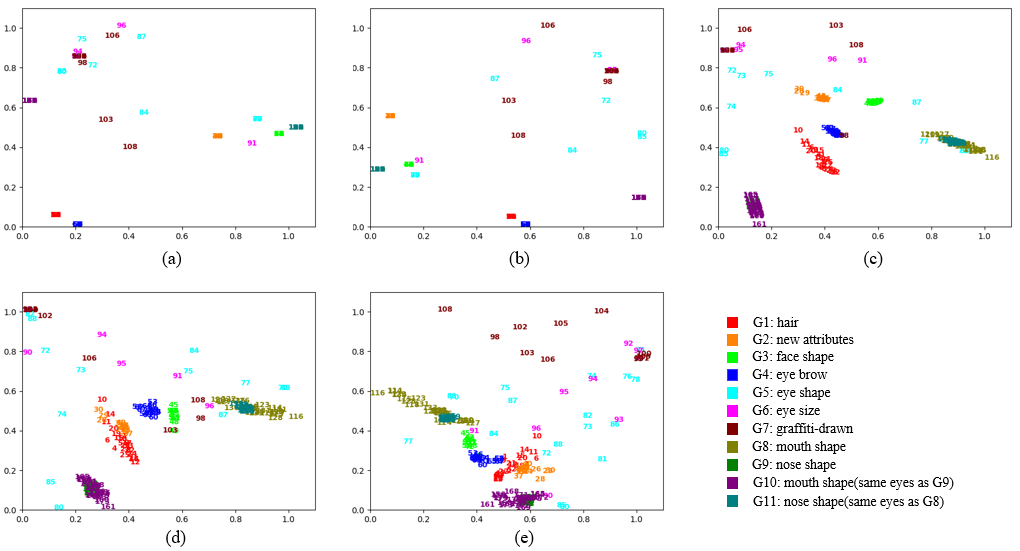
\includegraphics[width=0.8 \textwidth]{pca_1.png}
	\caption{Results of PCA visualization on $\boldsymbol{v}_0$ and $\boldsymbol{v}_1$}
	\label{fig:pca_1}
\end{figure*}


\subsection{Results}\label{sec:results}

%\section{About the paper submission}
%
%\subsection{Paper length}
%cvm papers may be between 4 pages and 14 pages. Over length papers will simply not be reviewed.
%
%%-------------------------------------------------------------------------
%\subsection{Draft and final copy}
%The \LaTeX\ style defines a printed ruler which should be present in the
%version submitted for review.  The ruler is provided in order that
%reviewers may comment on particular lines in the paper without
%circumlocution. The camera ready copy should not contain a ruler.
%(\LaTeX\ users may uncomment the \verb'\cvmfinalcopy' command in the document preamble.)
%
%\subsection{Blind review}
%Many authors misunderstand the concept of anonymizing for blind
%review.  Blind review does not mean that one must remove
%citations to one's own work---in fact it is often impossible to
%review a paper unless the previous citations are known and
%available.
%Blind review means that you do not use the words ``my'' or ``our''
%when citing previous work.
%
%%\begin{figure}[t]
%%\begin{center}
%%\fbox{\rule{0pt}{2in} \rule{0.9\linewidth}{0pt}}
%%   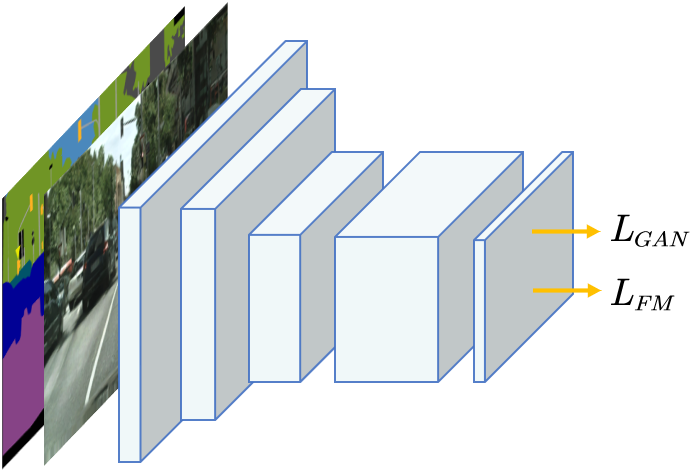
\includegraphics[width=0.8\linewidth]{pix2pixhd_D.png}
%%\end{center}
%%   \caption{Example of caption. }
%%\label{fig:long}
%%\label{fig:onecol}
%%\end{figure}
%
%\subsection{Miscellaneous}
%
%\noindent
%Compare the following:\\
%\begin{tabular}{ll}
% \verb'$conf_a$' &  $conf_a$ \\
% \verb'$\mathit{conf}_a$' & $\mathit{conf}_a$
%\end{tabular}\\
%See The \TeX book, p165.
%
%The space after \eg, meaning ``for example'', should not be a
%sentence-ending space. So \eg is correct, {\em e.g.} is not.  The provided
%\verb'\eg' macro takes care of this.
%
%When citing a multi-author paper, you may save space by using ``et alia'',
%shortened to ``\etal'' (not ``{\em et.\ al.}'' as ``{\em et}'' is a complete word.)
%However, use it only when there are three or more authors.  Thus, the
%following is correct: ``
%   Frobnication has been trendy lately.
%   It was introduced by Alpher~\cite{Alpher02}, and subsequently developed by
%   Alpher and Fotheringham-Smythe~\cite{Alpher03}, and Alpher \etal~\cite{Alpher04}.''
%
%This is incorrect: ``... subsequently developed by Alpher \etal~\cite{Alpher03} ...''
%because reference~\cite{Alpher03} has just two authors.  If you use the
%\verb'\etal' macro provided, then you need not worry about double periods
%when used at the end of a sentence as in Alpher \etal.
%
%For this citation style, keep multiple citations in numerical (not
%chronological) order, so prefer \cite{Alpher03,Alpher02,Authors12} to
%\cite{Alpher02,Alpher03,Authors12}.
%
%%-------------------------------------------------------------------------
%\subsection{References}
%
%List and number all bibliographical references in 9-point Times,
%single-spaced, at the end of your paper. When referenced in the text,
%enclose the citation number in square brackets, for
%example~\cite{Authors12}.  Where appropriate, include the name(s) of
%editors of referenced books.
%
%\begin{table}
%\begin{center}
%\begin{tabular}{|l|c|}
%\hline
%Name & Performance \\
%\hline\hline
%A & OK\\
%B & Bad \\
%Ours & Great\\
%\hline
%\end{tabular}
%\end{center}
%\caption{An example for using tables.}
%\end{table}
%
%%-------------------------------------------------------------------------
%\subsection{Illustrations, graphs, and photographs}
%
%All graphics should be centered.  Please ensure that any point you wish to
%make is resolvable in a printed copy of the paper.  Resize fonts in figures
%to match the font in the body text, and choose line widths which render
%effectively in print.  Many readers (and reviewers), even of an electronic
%copy, will choose to print your paper in order to read it.  You cannot
%insist that they do otherwise, and therefore must not assume that they can
%zoom in to see tiny details on a graphic.
%
%When placing figures in \LaTeX, it's almost always best to use
%\verb+\includegraphics+, and to specify the  figure width as a multiple of
%the line width as in the example below
%{\small\begin{verbatim}
%   \usepackage[dvips]{graphicx} ...
%   \includegraphics[width=0.8\linewidth]
%                   {myfile.eps}
%\end{verbatim}
%}
%
%
%%-------------------------------------------------------------------------
%
{\small
\bibliographystyle{cvm}
\bibliography{cvmbib}
}


\end{document}
